\section{Graph theory}
    \begin{frame}{Motivation}
        \begin{figure}[htp!]
            \centering
            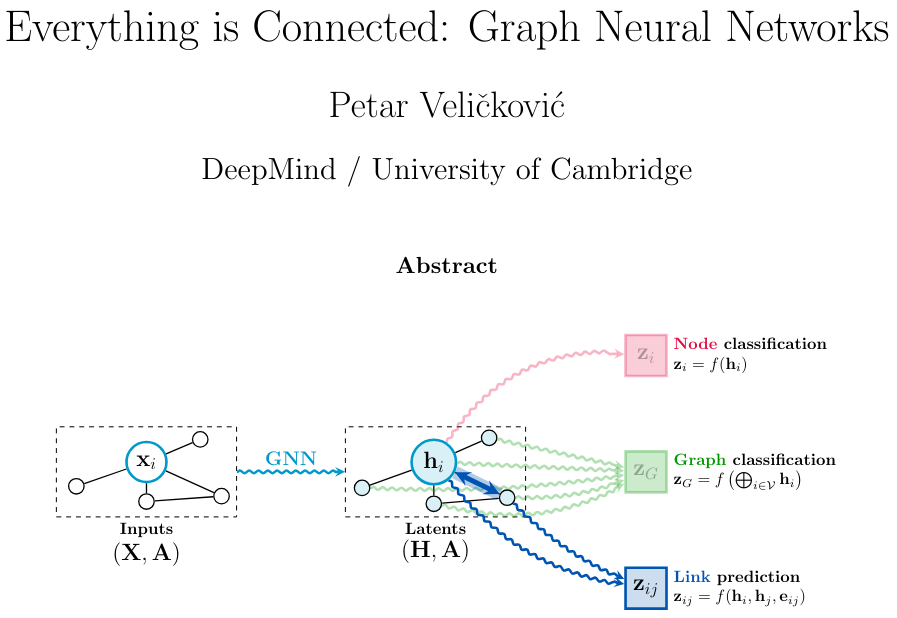
\includegraphics[
                width=0.6\linewidth,
                trim=0pt 0pt 0pt 0pt, % trim: left bottom right top.
                clip
            ]{../images/everything_is_connected.png}

            \caption{Everything is connected.}
            \vspace{-15pt}
            % \caption*{\tiny From: \url{https://www.researchgate.net/figure/Relationship-between-artificial-intelligence-machine-learning-neural-network-and-deep_fig3_354124420}} 
            \label{fig:everything_connected}
        \end{figure}

        \begin{note}
            {Introduce your self}
        \end{note}
    \end{frame}

    \begin{frame}{Graphs}
        In mathematics and computer science, a graph (network) is defined as $G = (V, E)$, where $V = \{v_1, v_2, ..., v_{n}\}$ is the nodes (or \textit{vertices}, or \textit{points}) set and $E = \{e_1, e_2, ..., e_{m}\}, e_i \in V \times V$ a set of edges (or \textit{lines}, or \textit{arcs}) formed by unordered pairs of nodes. \\

        \vspace{2mm}
        \scriptsize Number of nodes is denoted $|V|$. \\
        Number of edges is denoted $|E|$.

        \begin{figure}[ht!]
            \centering
            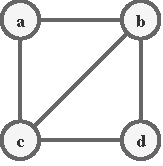
\includegraphics[width=0.25\linewidth]{../images/graph_example.pdf}
            \caption{Graph example.}
            \label{fig:graph_example}
        \end{figure}

        \begin{note}
            {Introduce your self}
        \end{note}
    \end{frame}

    \begin{frame}{Graphs}
        Furthermore, each edge $e \in E$ is said to join two vertices. If $e$ joins $u, v \in V$, then $e = (u, v)$. Vertices $u$ and $v$ are said to be adjacent. \\
        
        \begin{exampleblock}{Neighborhood}
            \begin{equation}
            \mathcal{N}(v) = \{w \in V \mid v \neq w \land (v, w) \in E\}
            \label{eq:neighborhood}
            \end{equation}
        \end{exampleblock}

        \begin{note}
            {Introduce your self}
        \end{note}
    \end{frame}

    \begin{frame}{Networks are everywhere!}
        \begin{figure}[ht!]
            \centering
            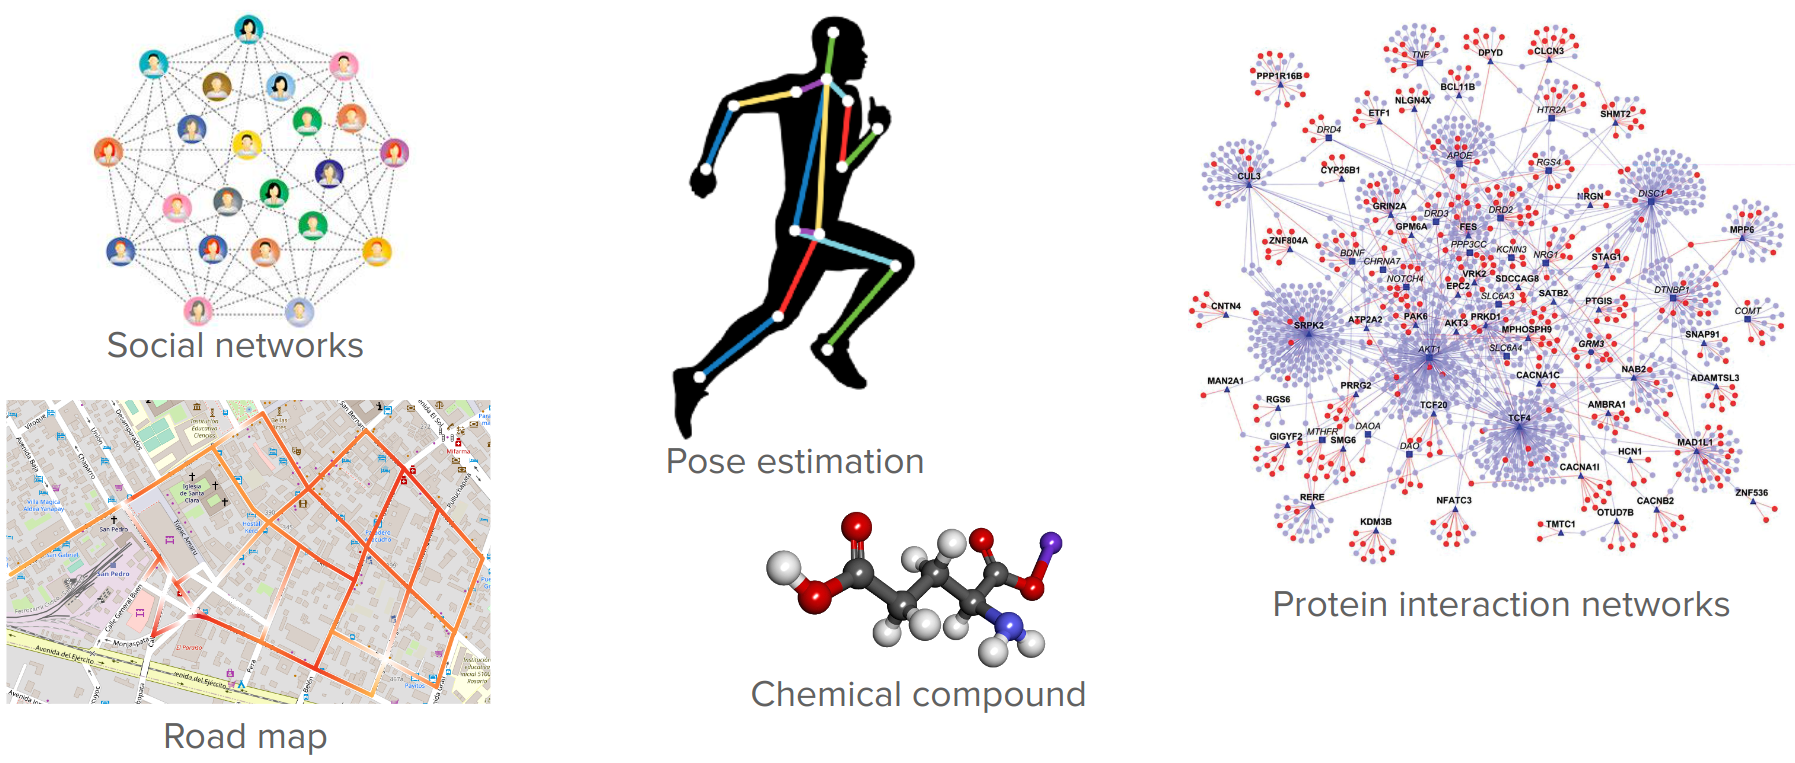
\includegraphics[width=1.0\linewidth]{../images/networks_everywhere.png}
            \caption{Networks examples.}
            \label{fig:networks_everywhere}
        \end{figure}

        \begin{note}
            {Introduce your self}
        \end{note}
    \end{frame}

    \begin{frame}{Networks are everywhere!}
        \begin{figure}[ht!]
            \centering
            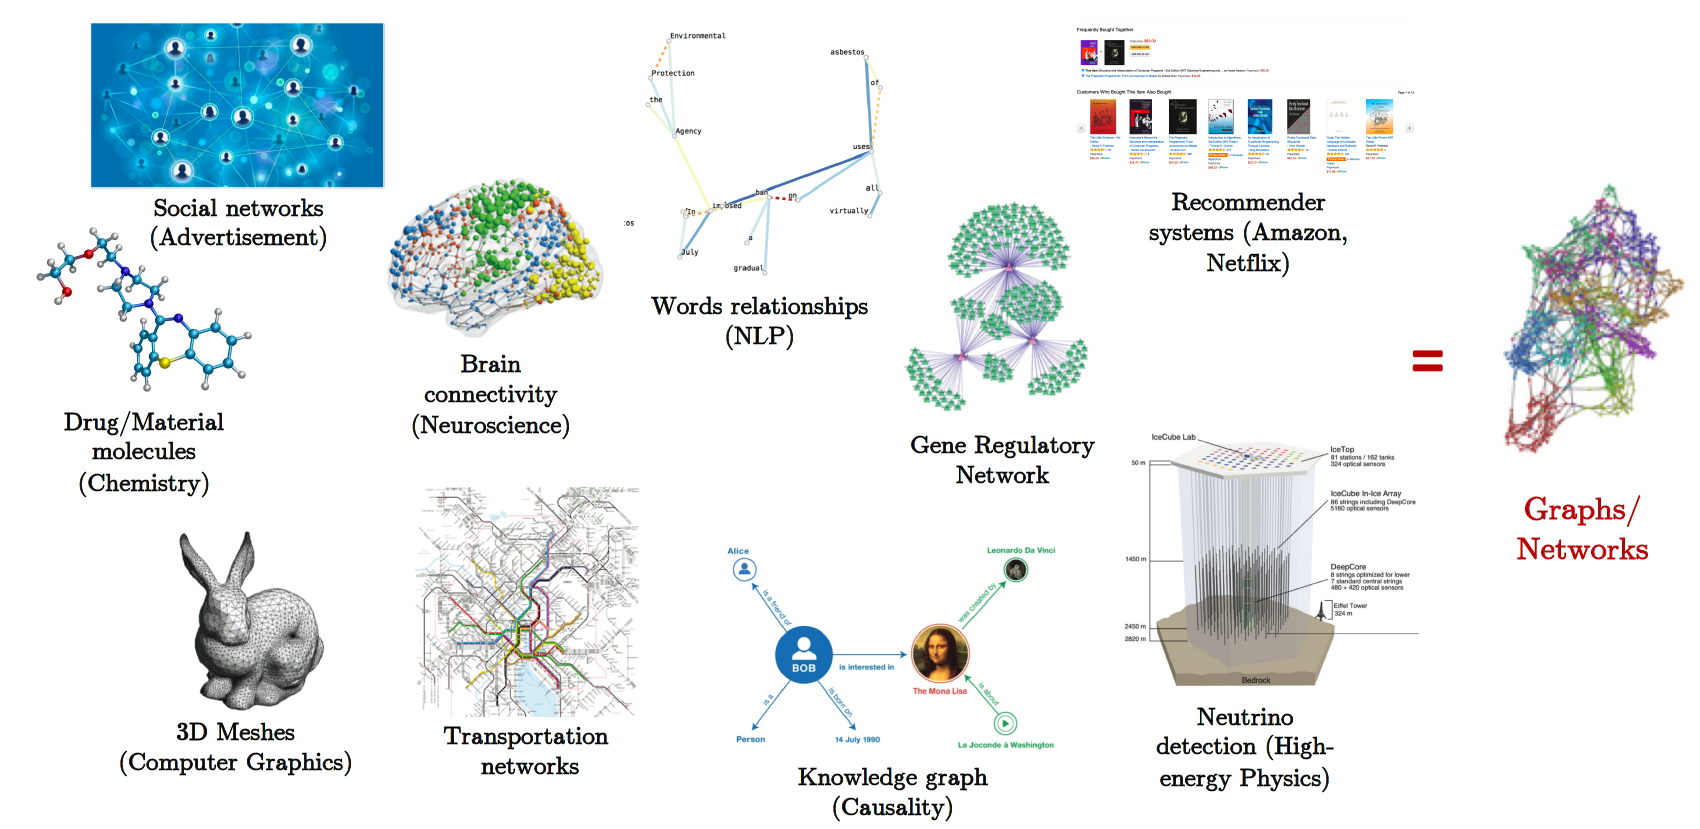
\includegraphics[width=1.0\linewidth]{../images/graph-data.png}
            \caption{\scriptsize Networks examples.}
            % From \url{https://graphdeeplearning.github.io/project/spatial-convnets/}.}
        \end{figure}
        
        \begin{note}
            {Introduce your self}
        \end{note}
    \end{frame}

    \begin{frame}{Graph representations}
        \begin{figure}
            \centering
            \begin{subfigure}{0.22\textwidth}
                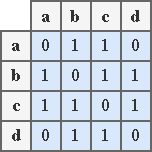
\includegraphics[width=\textwidth]{../images/graph_adjacency_matrix.pdf}
                \caption{Adjacency matrix.}
                \label{fig:graph_adjacency_matrix_}
            \end{subfigure}
            \hfill
            \begin{subfigure}{0.22\textwidth}
                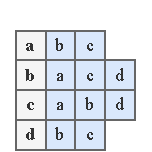
\includegraphics[width=\textwidth]{../images/graph_adjacency_list.pdf}
                \caption{Adjacency list.}
                \label{fig:graph_adjacency_list_}
            \end{subfigure}
            \hfill
            \begin{subfigure}{0.22\textwidth}
                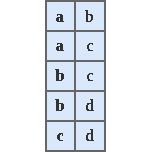
\includegraphics[width=\textwidth]{../images/graph_list_edge.pdf}
                \caption{Edge list.}
                \label{fig:graph_list_edge_}
            \end{subfigure}
            \hfill
            \begin{subfigure}{0.26\textwidth}
                
\includegraphics[width=\textwidth]{../images/incidence_matrix.pdf}
                \caption{Incidence matrix.}
                \label{fig:graph_incidence_matrix_}
            \end{subfigure}
            \hfill
            \begin{subfigure}{0.2\textwidth}
                
\includegraphics[width=\textwidth]{../images/graph_inc.pdf}
                \caption{Input graph.}
                \label{fig:graph_example_}
            \end{subfigure}
            \caption{Graph representations.}
            \label{fig:graph_representation_}
        \end{figure}

        \begin{note}
            {Write your notes here}
        \end{note}
    \end{frame}

    \begin{frame}{Graphs are everywhere!}
        \begin{figure}[ht!]
            \centering
            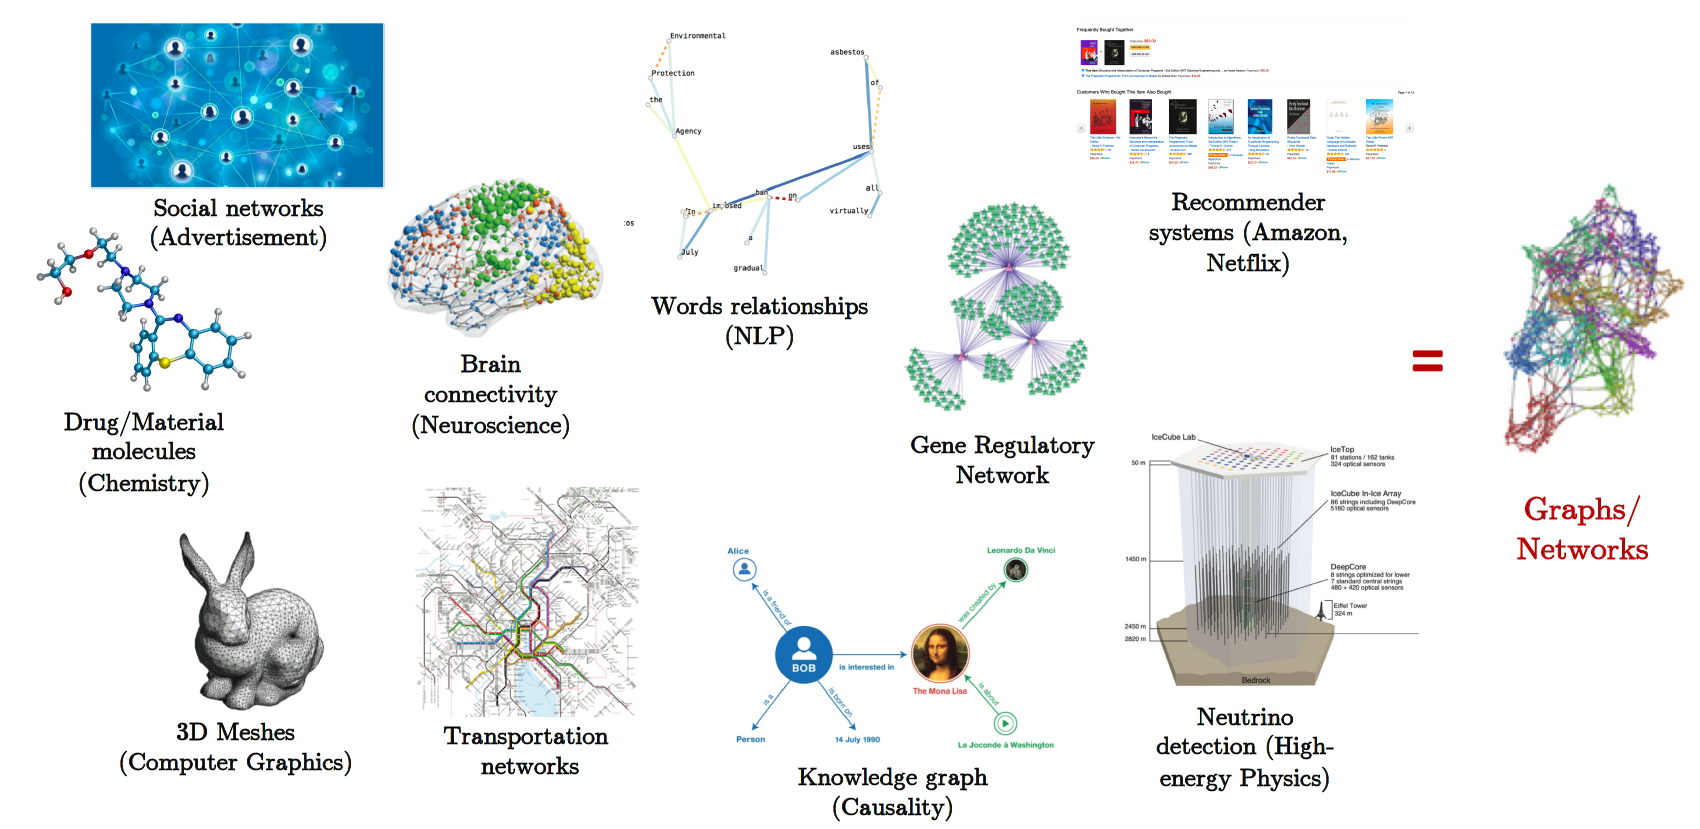
\includegraphics[width=1.0\linewidth]{../images/graph-data.png}
            \caption{Graphs are everywhere.}
            \vspace{-15pt}
            \caption*{\tiny From \url{https://graphdeeplearning.github.io/project/spatial-convnets/}}
            %%% \label{fig:most-used-social-platforms-worldwide} 
        \end{figure}               
    \end{frame}

    \begin{frame}{Types of graphs}
        \begin{columns}[t] % The "c" centered vertical alignment, "t" top vertical alignment
            \begin{column}{0.35\textwidth}
                \begin{itemize}
                    \item \alert{Based on nodes}
                    \begin{itemize}
                        \item Homogeneous
                        \item Heterogeneous
                    \end{itemize}
                \end{itemize}
            \end{column}
            
            \begin{column}{0.34\textwidth}
                \begin{itemize}
                    \item \alert{Based on edges}
                    \begin{itemize}
                        \item Undirected
                        \item Directed
                        \item Unweighted
                        \item Weighted
                        \item Sparse
                        \item Dense
                    \end{itemize}
                \end{itemize}
            \end{column}

            \begin{column}{0.32\textwidth}
                \begin{itemize}
                    \item \alert{Special types}
                    \begin{itemize}
                        \item Complete
                        \item Subgraph
                        \item Hypergraph
                        \item \textit{k}-partite
                        \item Acyclic and Cyclic
                        \item Tree
                        \item Knowledge            
                        % \item Planar
                    \end{itemize}
                \end{itemize}
            \end{column}
        \end{columns}

        \begin{note}
            {Introduce your self}
        \end{note}
    \end{frame}

    \begin{frame}{Types of graphs}
        \begin{figure}
            \centering
            \begin{subfigure}{0.241\textwidth}
                
\includegraphics[width=\textwidth]{../images/homogeneous_graph.pdf}
                \caption{Homogeneous.}
                %%% \label{fig:homogeneous_graph}
            \end{subfigure}
            \hfill
            \begin{subfigure}{0.241\textwidth}
                
\includegraphics[width=\textwidth]{../images/heterogeneous_graph.pdf}
                \caption{Heterogeneous.}
                %%% \label{fig:heterogeneous_graph}
            \end{subfigure}
            \hfill
            \begin{subfigure}{0.241\textwidth}
                
\includegraphics[width=\textwidth]{../images/directed_graph.pdf}
                \caption{Directed.}
                %%% \label{fig:directed_graph}
            \end{subfigure}
            \hfill
            \begin{subfigure}{0.241\textwidth}
                
\includegraphics[width=\textwidth]{../images/weighted_undirected_graph.pdf}
                \caption{Weighted.}
                %%% \label{fig:weighted_undirected_graph}
            \end{subfigure}
            \hfill
            \begin{subfigure}{0.16\textwidth}
                
\includegraphics[width=\textwidth]{../images/complete_graph.pdf}
                \caption{Complete.}
                %%% \label{fig:complete_graph}
            \end{subfigure}
            \hfill
            \begin{subfigure}{0.195\textwidth}
                
\includegraphics[width=\textwidth]{../images/tree.pdf}
                \caption{Tree.}
                %%% \label{fig:tree}
            \end{subfigure}
            \hfill
            \begin{subfigure}{0.11\textwidth}
                
\includegraphics[width=\textwidth]{../images/2_partite_graph.pdf}
                \caption{Bipartite.}
                %%% \label{fig:2_partite_graph}
            \end{subfigure}
            \hfill
            \begin{subfigure}{0.25\textwidth}
                
\includegraphics[width=\textwidth]{../images/knowledge_graph.pdf}
                \caption{Knowledge.}
                %%% \label{fig:knowledge_graph}
            \end{subfigure}
            \caption{Types of graphs.}
            %%% \label{fig:types_graphs}
        \end{figure}                     
    \end{frame}
    
    % \begin{frame}{Based on nodes}         
    %     \begin{exampleblock}{Homogeneous graph}
    %         Is a graph $G = (V, E)$ in which all nodes and/or edges are of the same type, or class. %, meaning they represent entities of the same class or category, and there is no distinction.
            
    %         \begin{figure}[ht!]
    %             \centering
    %             
\includegraphics[width=0.4\linewidth]{../images/homogeneous_graph.pdf}
    %             \caption{Homogeneous graph.}
    %             %%% \label{fig:homogeneous_graph}
    %         \end{figure}
    %     \end{exampleblock}
    %     \vspace{-2mm}

    %     % Example: In a social network, where all vertices represent people and edges represent friendships.
        
    %     \begin{note}
    %         {Introduce your self}
    %     \end{note}
    % \end{frame}

    % \begin{frame}{Based on nodes}         
    %     \begin{exampleblock}{Heterogeneous graph}
    %         Is a graph $G = (V, E)$ in which nodes and/or edges belong to different types or classes. % In such graphs, vertices represent different kinds of entities, and edges represent different types of relationships.
            
    %         \begin{figure}[ht!]
    %             \centering
    %             
\includegraphics[width=0.4\linewidth]{../images/heterogeneous_graph.pdf}
    %             \caption{Heterogeneous graph.}
    %             %%% \label{fig:heterogeneous_graph}
    %         \end{figure}
    %     \end{exampleblock}
    %     \vspace{-2mm}

    %     % Example: In a social school network, where nodes represent teachers/students and edges represent friendships.
        
    %     \begin{note}
    %         {Introduce your self}
    %     \end{note}
    % \end{frame}

    % \begin{frame}{Based on edges}         
    %     \begin{exampleblock}{Directed graph (digraph)}
    %         Is a graph $G = (V, E)$ in which each edge has a direction. 
    %         An edge $(u, v)$ is not the same as $(v, u)$.
    %         % Formally, edges are represented as ordered pairs $(u, v)$, indicating a connection from node $u$ to node $v$. 
    %         % E⊆V×V is a set of ordered pairs called arcs or directed edges
            
    %         \begin{figure}[ht!]
    %             \centering
    %             
\includegraphics[width=0.4\linewidth]{../images/directed_graph.pdf}
    %             \caption{Directed graph.}
    %             %%% \label{fig:directed_graph}
    %         \end{figure}
    %     \end{exampleblock}
    %     \vspace{-2mm}

    %     % Example: commonly used to model asymmetric relationships, such as: follow relationships in social networks, task dependencies, etc.

    %     \begin{note}
    %         {Introduce your self}
    %     \end{note}
    % \end{frame}

    % \begin{frame}{Based on edges}         
    %     \begin{exampleblock}{Weighted graph}
    %         Is a graph $G = (V, E, w)$ in which each edge is assigned a numerical value, called a weight. This weight is denoted $w(u, v)$ for edge $(u, v)$.
    %         % $G = (V, E, w)$
            
    %         \begin{figure}
    %             \centering
    %             \begin{subfigure}{0.4\textwidth}
    %                 
\includegraphics[width=\textwidth]{../images/weighted_undirected_graph.pdf}
    %                 \caption{Weighted \& undirected.}
    %                 %%% \label{fig:weighted_undirected_graph}
    %             \end{subfigure}
    %             % \hfill
    %             \hspace{1cm}
    %             \begin{subfigure}{0.4\textwidth}
    %                 
\includegraphics[width=\textwidth]{../images/weighted_directed_graph.pdf}
    %                 \caption{Weighted \& undirected.}
    %                 %%% \label{fig:weighted_directed_graph}
    %             \end{subfigure}
    %             \caption{Weighted graph.}
    %             %%% \label{fig:weighted_graph}
    %         \end{figure}
    %     \end{exampleblock}
    %     \vspace{-2mm}
        
    %     % Example: commonly used in shortest path problems, network routing, road maps, cost optimization problems, etc.

    %     \begin{note}
    %         {Introduce your self}
    %     \end{note}
    % \end{frame}

    % % Complete graph
    % \begin{frame}{Special types}         
    %     \begin{exampleblock}{Complete graph}
    %         % A simple graph G is complete if every pair of distinct vertices is adjacent. The complete graph on n vertices is denoted Kn.

    %         A complete graph $G = (V, E)$ is a simple graph in which each pair of distinct vertices is adjacent to each other. In other words, there are all possible edges between the nodes.
            
    %         \begin{figure}[ht!]
    %             \centering
    %             
\includegraphics[width=0.27\linewidth]{../images/complete_graph.pdf}
    %             \caption{Complete graph.}
    %             %%% \label{fig:complete_graph}
    %         \end{figure}
    %     \end{exampleblock}
    %     \vspace{-5mm}
        
    %     % Example: In modeling networks with maximum connectivity, etc.

    %     \begin{note}
    %         {Introduce your self}
    %     \end{note}
    % \end{frame}

    % % Subgraph graph
    % \begin{frame}{Special types}         
    %     \begin{exampleblock}{Subgraph graph}
    %         A subgraph of a graph $G_1 = (V_1, E_1)$ is a graph $G_2 = (V_2, E_2)$ that satisfies $V_2 \subseteq V_1$ and $E_2 \subseteq E_1$.%  \cite{saoub2021graph}.
            
    %         %  A subgraph H of a graph G is a graph where H contains some of the edges and vertices of G; that is, V (H) ⊆ V (G) and E(H) ⊆ E(G).

    %         \begin{figure}
    %             \centering
    %             \begin{subfigure}{0.41\textwidth}
    %                 
\includegraphics[width=\textwidth]{../images/homogeneous_graph}
    %                 \caption{Graph $G_{1}$.}
    %                 %%% \label{fig:graph}
    %             \end{subfigure}
    %             % \hfill
    %             \hspace{1cm}
    %             \begin{subfigure}{0.18\textwidth}
    %                 
\includegraphics[width=\textwidth]{../images/subgraph.pdf}
    %                 \caption{Subgraph $G_{2}$.}
    %                 %%% \label{fig:subgraph}
    %             \end{subfigure}
    %             \caption{Graph and subgraph.}
    %             %%% \label{fig:graph_subgraph}
    %         \end{figure}

    %         % Example: In a social network, where all vertices represent people and edges represent friendships.
    %     \end{exampleblock}

    %     \begin{note}
    %         {Introduce your self}
    %     \end{note}
    % \end{frame}

    % % Tree
    % \begin{frame}{Special types}         
    %     \begin{exampleblock}{Tree}
    %         % A simple, connected graph having no cycles is called a tree. A simple graph having only trees as its components, is called a forest.
    %         % For any connected (simple) graph G with n vertices and m edges, n ≤ m + 1.
    %         A graph $G = (V, E)$ is a tree if and only if there exists exactly one path between every two vertices $u$ and $v$.
            
    %         \begin{figure}[ht!]
    %             \centering
    %             
\includegraphics[width=0.37\linewidth]{../images/tree.pdf}
    %             \caption{Tree.}
    %             %%% \label{fig:tree}
    %         \end{figure}
    %     \end{exampleblock}
    %     \vspace{-5mm}

    %     % Example: In data structures, file system, machine learning, etc.

    %     \begin{note}
    %         {Introduce your self}
    %     \end{note}
    % \end{frame}

    % % Knowledge graph
    % \begin{frame}{Special types}         
    %     \begin{exampleblock}{Knowledge graph}
    %         A knowledge graph (KG) is a labeled directed graph, where the nodes represent the entities and the edges represent the semantic relationships between them.
    %         \footnotesize KG is defined as a set of triplets: $\text{KG} = \{(s, p, o) | s \in \mathscr{E}, p \in \mathscr{R}, o \in \mathscr{E}\}$. Where, $s$ a subject (an entity), $p$ a predicate (a relation), $o$ an object (an entity), $\mathscr{E}$ set of entities (nodes), $\mathscr{R}$ set of relations (edge labels).
            
    %         % relationships between them.
    %         \begin{figure}[ht!]
    %             \centering
    %             
\includegraphics[width=0.45\linewidth]{../images/knowledge_graph.pdf}
    %             \caption{Knowledge graph.}
    %             %%% \label{fig:knowledge_graph}
    %         \end{figure}
    %     \end{exampleblock}
    %     \vspace{-5mm}

    %     % Example: In question-answering systems, healthcare, recommender systems, etc.
        
    %     \begin{note}
    %         {Introduce your self}
    %     \end{note}
    % \end{frame}

    \begin{frame}{What type of graph is this?}
        \begin{figure}
            \centering
            \begin{subfigure}{0.26\textwidth}
                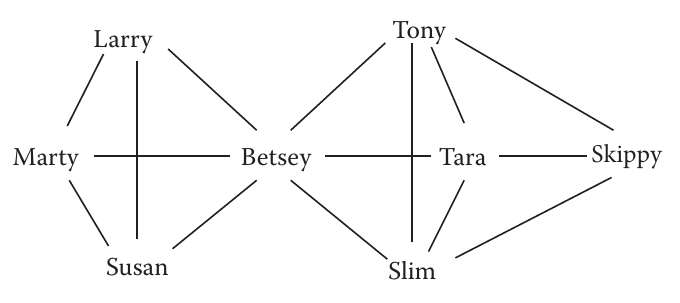
\includegraphics[width=\textwidth]{../images/social_networks.png}
                \caption{Social networks.}
                %\label{fig:social_networks}
            \end{subfigure}
            % \hfill
            \begin{subfigure}{0.27\textwidth}
                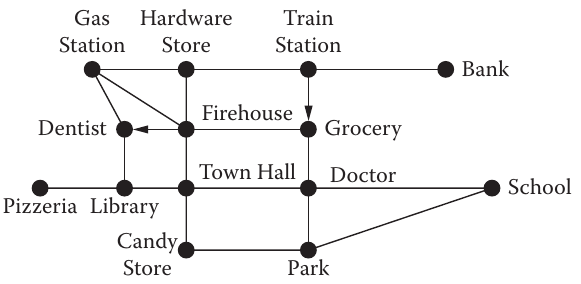
\includegraphics[width=\textwidth]{../images/road_map_landmarks.png}
                \caption{Road-map networks.}
                % \label{fig:road_map_landmarks}
            \end{subfigure}
            % \hfill
            \begin{subfigure}{0.22\textwidth}
                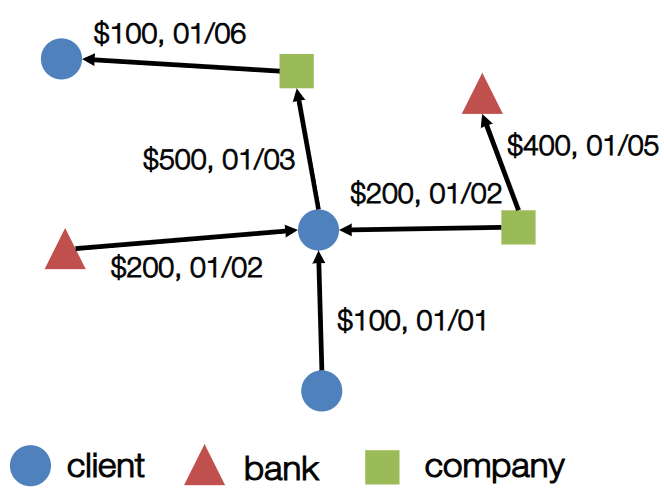
\includegraphics[width=\textwidth]{../images/financial_networks.png}
                \caption{Financial networks.}
                % \label{fig:financial_networks}
            \end{subfigure}
            % hfill
            \begin{subfigure}{0.18\textwidth}
                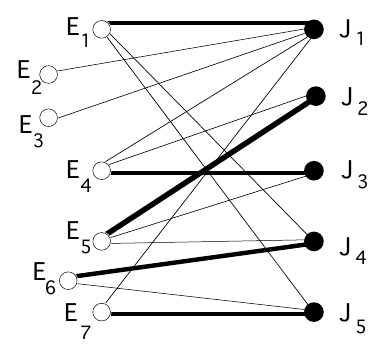
\includegraphics[width=\textwidth]{../images/personnel_assignment.png}
                \caption{Employee–job networks.}
                % \label{fig:personnel_assignment}
            \end{subfigure}
            \caption{Graphs are everywhere.}
            %\label{fig:graph_everywhere}
        \end{figure}                     
    \end{frame}

    \begin{frame}{Algorithms on graphs}
        \begin{columns}[t] % The "c" centered vertical alignment, "t" top vertical alignment
            \begin{column}{0.45\textwidth}
                \begin{itemize}
                    \item \alert{Network traversal}
                    \begin{itemize}
                        \item Breadth-First Search
                        \item Depth-First Search
                    \end{itemize}
                \end{itemize}
            \end{column}
            
            \begin{column}{0.55\textwidth}
                \begin{itemize}
                    \item \alert{Shortest path algorithms}
                    \begin{itemize}
                        \item Dijkstra
                        \item Floyd–Warshall
                        \item Bellman-Ford
                    \end{itemize}
                \end{itemize}
            \end{column}
        \end{columns}

        \begin{note}
            {Introduce your self}
        \end{note}
    \end{frame}

    \begin{frame}{Breadth-First Search (BFS) algorithm}        
        \begin{columns}[t] % The "c" option specifies centered vertical alignment while the "t" option is used for top vertical alignment
            \begin{column}{0.6\textwidth}
                \begin{enumerate}
                    \item Visit the adjacent unvisited node. Mark as visited, display, and insert (queue) in a queue.
                    \item In case no adjacent node is found, remove the first node from the queue.
                    \item Repeat steps 1, and 2 until the queue is empty.
                \end{enumerate}
            \end{column}
            
            \begin{column}{0.4\textwidth}
                \begin{figure}[ht!]
                    \centering
                    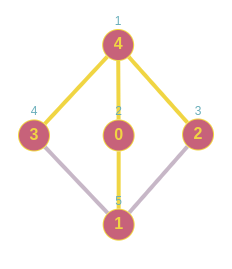
\includegraphics[width=0.8\linewidth]{../images/bfs_v1.png}
                    \caption{BFS traversal from node 4 are 4, 0, 2, 3, 1.}
                    % \caption*{Adapted from \cite{labonne2023hands}.}
                    \label{fig:bfs}
                \end{figure}
            \end{column}
        \end{columns}
        
        \begin{note}
            {Introduce your self}
        \end{note}
    \end{frame}

    \begin{frame}{Depth-First Search (DFS) algorithm}
        \begin{columns}[t] % The "c" option specifies centered vertical alignment while the "t" option is used for top vertical alignment
            \begin{column}{0.6\textwidth}
                \begin{enumerate}
                    \item Visit the adjacent unvisited node. Mark as visited, show, and push in a stack.
                    \item In case no adjacent nodes are found, all nodes in the stack that do not have adjacent nodes are popped.
                    \item Repeat steps 1, and 2 until the stack is empty.
                \end{enumerate}
            \end{column}
            
            \begin{column}{0.4\textwidth}
                \begin{figure}[ht!]
                    \centering
                    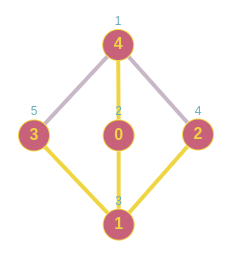
\includegraphics[width=0.7\linewidth]{../images/dfs_v1.png}
                    \caption{DFS traversal from node 4 are 4, 0, 1, 2, 3.}
                    % \caption*{Adapted from \cite{labonne2023hands}.}
                    \label{fig:dfs}
                \end{figure}
            \end{column}
        \end{columns}
        
        \begin{note}
            {Introduce your self}
        \end{note}
    \end{frame}

    \begin{frame}{Example}
        \begin{figure}[ht!]
            \centering
            
\includegraphics[width=0.3\linewidth]{../images/union.pdf}
            \caption{Input graph.}
            % \caption*{Adapted from \cite{labonne2023hands}.}
            \label{fig:union}
        \end{figure}
        
        \begin{note}
            {Introduce your self}
        \end{note}
    \end{frame}

    \begin{frame}{Dijkstra's Algorithm}
        Dijkstra's algorithm finds the shortest path from a source node to all other nodes in a directed or undirected graph with non-negative edge weights. \newline

        \begin{exampleblock}{Idea}
            Does the shortest path from $a$ to $c$ go through $b$?
            
            \begin{figure}[ht!]
                \centering
                
\includegraphics[width=0.25\linewidth]{../images/dijkstra_idea.pdf}
                \caption{Shortest path example.}
                %%% \label{fig:dijkstra_idea}
            \end{figure}
        \end{exampleblock}
        
        % Description:
        % \begin{itemize}
        %    \item Uses a priority queue to select the closest unvisited node.
        %    \item Maintains the minimum known distance to each node.
        %    \item It is a weighted generalization of BFS.
        % \end{itemize}

        \begin{note}
            {Introduce your self}
        \end{note}
    \end{frame}

    \begin{frame}{GPS navigation and maps application}
        \begin{figure}[htp!]
            \centering
            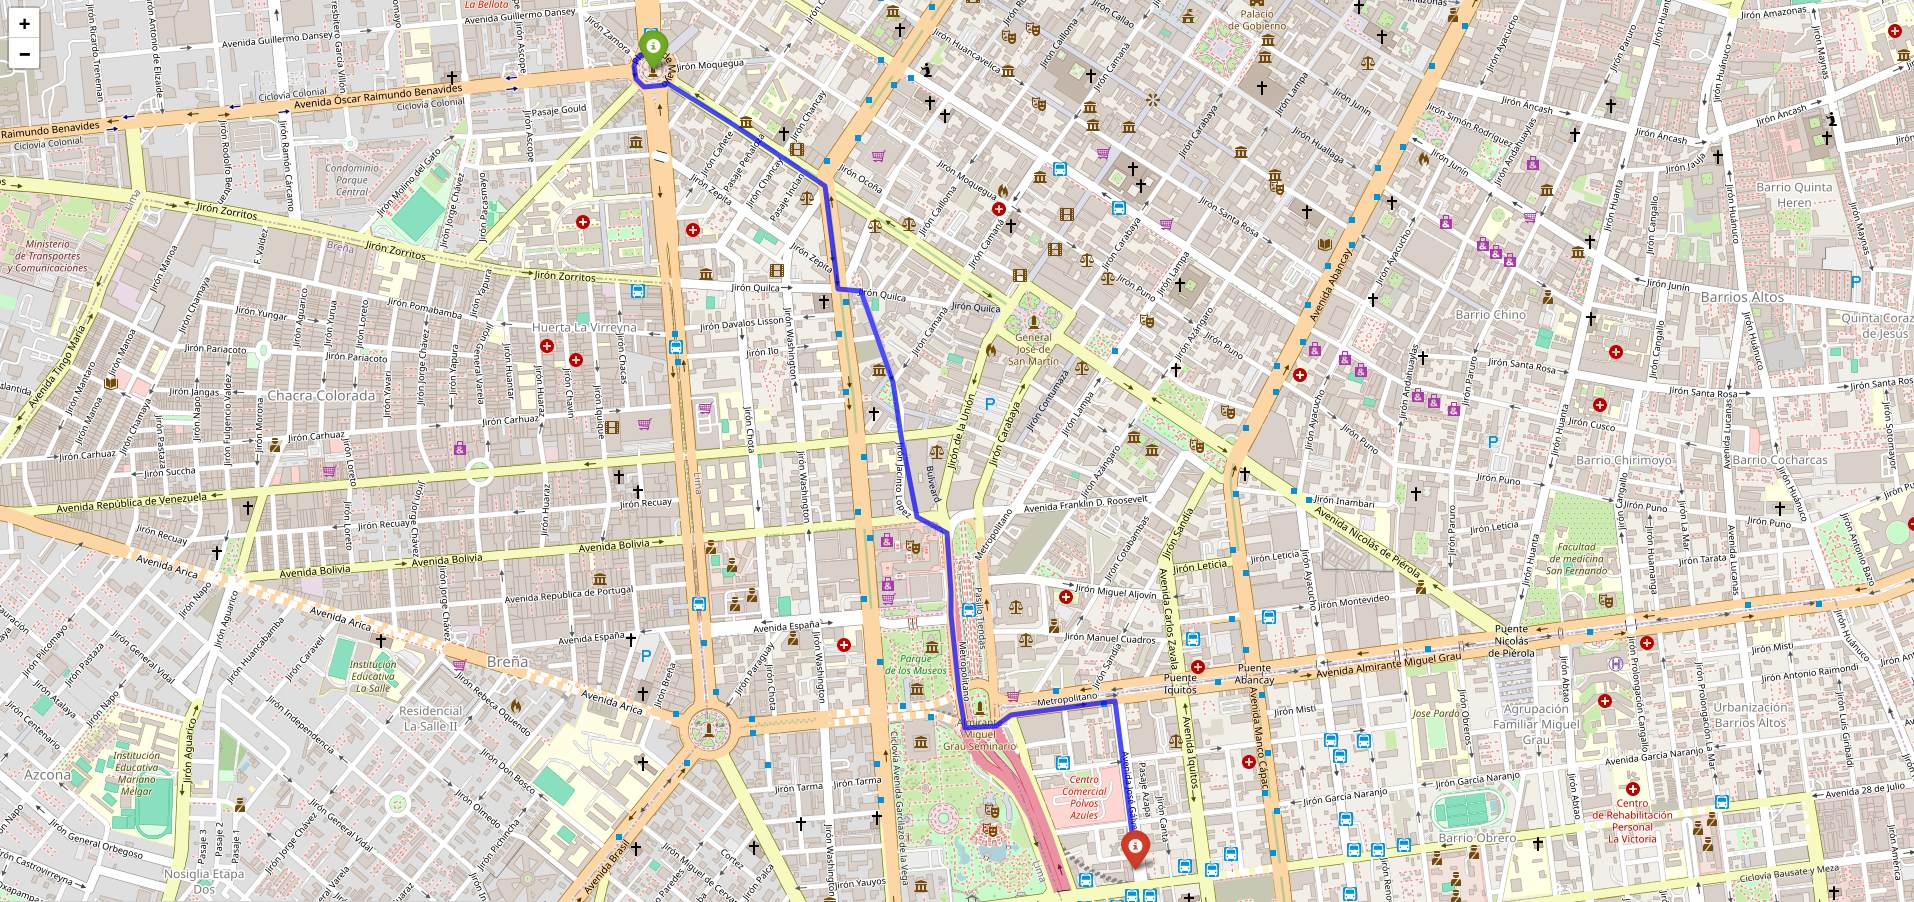
\includegraphics[width=0.9\linewidth]{../images/example_dijktra.png}
            \caption{Shortest path between two locations.}
            \label{fig:example_dijktra}
        \end{figure}

        \begin{note}
            {Introduce your self}
        \end{note}
    \end{frame}
    
    \begin{frame}{Metrics on graphs}
        \begin{columns}[t] % Option "c" centers vertically, while "t" aligns to the top.
            \begin{column}{0.33\textwidth}
                \begin{itemize}
                    \item \alert{Node-level}
                    \begin{itemize}
                        \item Degree
                        \item Degree distribution
                        \item Degree centrality
                        \item Closeness centrality
                        \item Betweenness centrality
                        % \item Centrality
                        \item Eccentricity
                        \item LCC
                    \end{itemize}
                \end{itemize}
            \end{column}
            \begin{column}{0.33\textwidth}
                \begin{itemize}
                    \item \alert{Edge-level}
                    \begin{itemize}
                        \item Shortest path
                        \item Betweenness centrality
                        \item Jaccard coefficient
                        % \item Distance
                    \end{itemize}
                \end{itemize}
            \end{column}
            \begin{column}{0.33\textwidth}
                \begin{itemize}
                    \item \alert{Graph-level}
                    \begin{itemize}
                        \item Order
                        \item Size
                        \item Density
                        \item Diameter
                        \item Radius
                        \item Average degree
                        \item Average LCC
                        \item GCC
                        \item Modularity
                    \end{itemize}
                \end{itemize}
            \end{column}
        \end{columns}

        \begin{note}
            {Introduce your self}
        \end{note}
    \end{frame}

    \begin{frame}{Node-level}
        \begin{exampleblock}{Degree}
            Given a graph $G = (V, E)$.
            
            % Number of edges incident to a node. \\

            The degree of a node $u$, denoted as $deg(u)$, is defined as the number of edges that are adjacent to this node $u$.
        \end{exampleblock}

        \begin{multicols}{2} % Two columns
            Undirected graphs:
            \begin{equation}
                deg(u) = |\{v \in V : (u, v) \in E\}|
                % \label{eq:my_equation}
            \end{equation}
        
            Directed graphs:
            \begin{equation}
                deg(u) = deg^{in}(u) + deg^{out}(u)
                % \label{eq:my_equation}
            \end{equation}
        \end{multicols}
        
        Where, $deg^{in}(u)$: in-degree and $deg^{out}(u)$: out-degree. \newline

        Applications:
        \begin{itemize}
            \item Social networks: users with many connections.
            \item Biology networks: metabolites involved in many reactions.
            \item Web: most linked pages.
        \end{itemize}

        \begin{note}
            {Introduce your self}
        \end{note}
    \end{frame}

    \begin{frame}{Node-level}
        \begin{exampleblock}{Degree distribution}
            Given a graph $G = (V, E)$.
            
            The degree distribution of a graph $G$ is the ratio of the number of nodes with degree $k$ to the total number of nodes.
        \end{exampleblock}

        \begin{equation}
            P(k) = \frac{|V|_{k}}{|V|}
            % \label{eq:my_equation}
        \end{equation}
        
        Applications:
        \begin{itemize}
            \item Social networks: detect hubs or influencers.
            \item Biological networks:  identify essential genes or proteins.
            \item Epidemiology: predict how diseases spread over networks.
        \end{itemize}

        \begin{note}
            {Introduce your self}
        \end{note}
    \end{frame}

    \begin{frame}{Node-level}
        \begin{exampleblock}{Betweenness centrality}
            Given a graph $G = (V, E)$.
            
            Betweenness centrality counts the number of times a particular node occurs on the shortest paths between other nodes.
            % While degree and closeness centralities are based on the concept of the person’s reachability, betweenness centrality, on the other hand, relies on the idea that a person is more important if he/she is more intermediary in the network.
        \end{exampleblock}

        \begin{equation}
            % BC(v) = {\sum_{s, t \in V,\, s \neq v \neq  t} \frac{\sigma(s, t | v)}{\sigma(s, t)}}
            BC(v) = \sum_{\substack{s,\, t \in V \\ s \neq v \neq t}} \frac{\sigma(s, t \mid v)}{\sigma(s, t)}
            % \label{eq:my_equation}
        \end{equation}

        Where $\sigma(s, t)$ is the total number of shortest paths between nodes $s$ and $t$, and $\sigma(s, t | v)$ is the total number of shortest paths between nodes $s$ and $t$ that passing through $v$. \newline
        
        Applications:
        \begin{itemize}
            \item Identifying bottlenecks or bridges in networks.
            \item Network security: Identify critical nodes for communication.
        \end{itemize}

        \begin{note}
            {Introduce your self}
        \end{note}
    \end{frame}

    \begin{frame}{Example}
        \begin{figure}[ht!]
            \centering
            
\includegraphics[width=0.3\linewidth]{../images/union.pdf}
            \caption{Input graph.}
            % \caption*{Adapted from \cite{labonne2023hands}.}
            \label{fig:union}
        \end{figure}
        
        \begin{note}
            {Introduce your self}
        \end{note}
    \end{frame}

    \begin{frame}{Edge-level}
        \begin{exampleblock}{Shortest path}
            Given a graph $G = (V, E)$.
            
            Shortest path between two nodes in a graph is the path with the minimum total weight.
        \end{exampleblock}
        
        Algorithms:
        \begin{itemize}
            \item Dijkstra's algorithm: for graphs with non-negative weights.
            \item Bellman-Ford: handles negative weights.
            \item Floyd-Warshall: all-pairs shortest paths.
        \end{itemize}

        Applications:
        \begin{itemize}
            \item GPS/Navigation systems: find the fastest or shortest route.
            \item Internet routing: determine optimal data transmission paths.
            \item Social networks: degrees of separation between people.
            \item Biology: identify efficient biochemical or signaling pathways.
        \end{itemize}

        \begin{note}
            {Introduce your self}
        \end{note}
    \end{frame}

    \begin{frame}{Edge-level}
        \begin{exampleblock}{Betweenness centrality}
            Given a graph $G = (V, E)$.
            
            Betweenness centrality of an edge $e$ is the ratio of the shortest paths that run through $e$ to the total number of shortest paths in $G$.
        \end{exampleblock}

        \begin{equation}
            BC(e) = {\sum_{s, t \in V ,\, s \neq t} \frac{\sigma(s, t | e)}{\sigma(s, t)}}
            % \label{eq:my_equation}
        \end{equation}

        Here, $\sigma(s, t)$ is the total number of shortest paths between nodes $s$ and $t$, and $\sigma(s, t | e)$ is the number of those paths passing through $e$. \newline
        
        Applications:
        \begin{itemize}
            \item Network robustness: identify critical connections.
            \item Community detection: find bridges between clusters.
            % \item Traffic networks: detect congestion points.
            \item Social networks: find communication bottlenecks.
        \end{itemize}

        \begin{note}
            {Introduce your self}
        \end{note}
    \end{frame}

    \begin{frame}{Graph-level}
        \begin{exampleblock}{Order}
            Given a graph $G = (V, E)$.
            
            The order of a graph $G$, denoted by $|V|$, is defined as the number of nodes in the graph $G$.
        \end{exampleblock}

        \begin{note}
            {Introduce your self}
        \end{note}
    \end{frame}

    \begin{frame}{Graph-level}
        \begin{exampleblock}{Size}
            Given a graph $G = (V, E)$.
            
            The size of a graph $G$, denoted by $|E|$, is defined as the number of edges in the graph $G$.
        \end{exampleblock}

        \begin{note}
            {Introduce your self}
        \end{note}
    \end{frame}

    \begin{frame}{Graph-level}
        \begin{exampleblock}{Density}
            Given a graph $G = (V, E)$.
            
            Density is defined as the number of network edges divided by the maximum possible number of edges between nodes in that network. All density values are between $0$ and $1$.
        \end{exampleblock}

        \begin{equation}
            D(G) = \frac{2|E|}{|V|(|V| - 1)}
            % \label{eq:my_equation}
        \end{equation}

        Applications:
        \begin{itemize}
            \item Comparing different networks.
            \item Analyzing how sparse or dense a system is.
        \end{itemize}

        \begin{note}
            {Introduce your self}
        \end{note}
    \end{frame}

    \begin{frame}{Example}
        \begin{figure}[ht!]
            \centering
            
\includegraphics[width=0.3\linewidth]{../images/union.pdf}
            \caption{Input graph.}
            % \caption*{Adapted from \cite{labonne2023hands}.}
            \label{fig:union}
        \end{figure}
        
        \begin{note}
            {Introduce your self}
        \end{note}
    \end{frame}

    \begin{frame}{Practical example: Graphs, representations and visualization}
        \begin{itemize}
            \item Install requirements
                \begin{itemize}
                    \item \texttt{Python}
                    \item \texttt{Pandas}
                    \item \texttt{Numpy}
                    \item \texttt{NetworkX}
                    \item \texttt{Matplotlib}
                \end{itemize}
            \item Topics 
                \begin{itemize}
                    \item Create networks
                    \item Metrics on networks
                    \item Networks visualization
                \end{itemize}
            \item Lab
                \begin{itemize}
                    \item              
                        \href{https://drive.google.com/file/d/199QkU5jbJrrg4URuxGU8wGuvIF91y1mo/view?usp=sharing}{
                            \beamergotobutton{\faGoogle\ Open in Google Colab}
                        }
                \end{itemize}
        \end{itemize}
    \end{frame}


\section{Applications}
    \begin{frame}{Applications}
        \begin{multicols}{2}
            \begin{itemize}
                \item Computer vision
                \item Natural language processing
                \item Recommender systems
                \item Program analysis
                \item Knowledge graphs
                \item Bioinformatics
                \item Chemistry
                \item Biology
                \item Physic
                \item Anomaly detection
                \item Urban intelligence
                \item Financial transaction
                \item ...
            \end{itemize}
        \end{multicols}          
    \end{frame}

    \begin{frame}{Application in computer vision}
        SuperGlue: Learning Feature Matching with Graph Neural Networks \cite{sarlin2020superglue}.
        
        \begin{figure}[ht!]
            \centering
            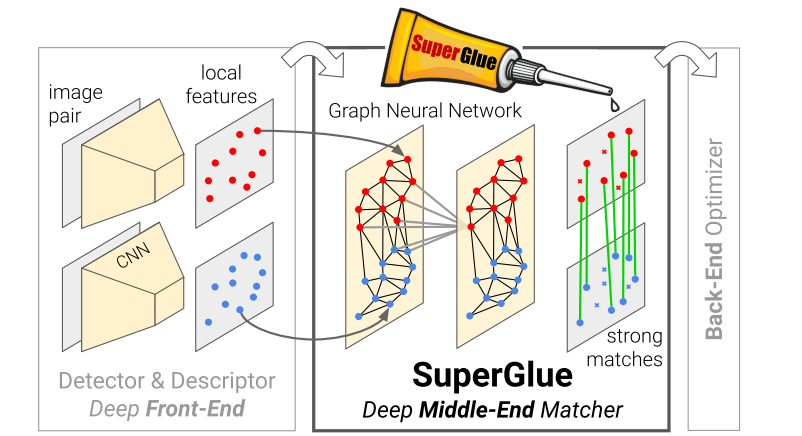
\includegraphics[width=0.7\linewidth]{../images/super_glue.png}
            \caption{SuperGlue scheme.}
        \end{figure}
    \end{frame}
    
    \begin{frame}{SuperGlue in action}
        \begin{figure}
            \centering
            % \includegraphics{}
            \animategraphics[width=\textwidth, loop, autoplay]
            {5} % frame rate
            {../images/imd/freiburg_matches-} % path to figures
            {0} % start index
            {15} % end index
            \caption{Matching example (indoor).}
            %%% \label{fig:app_superglue}
        \end{figure}
    \end{frame}

    \begin{frame}{SuperGlue in action}
        \begin{figure}[ht!]
            \centering
            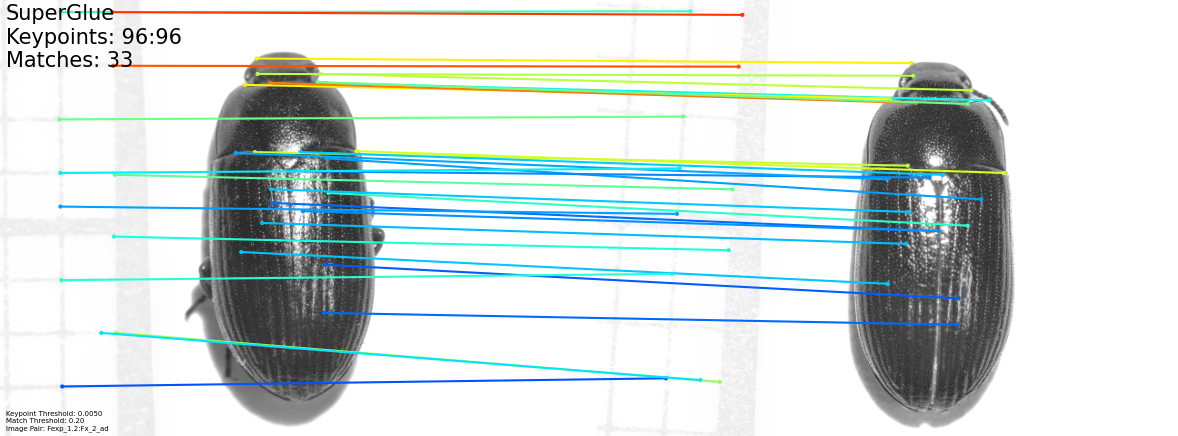
\includegraphics[width=1.0\linewidth]{../images/Fexp_1.2_Fx_2_ad_matches.png}
            \caption{Morphology of insects.}
        \end{figure}
    \end{frame}

    \begin{frame}{Application in urban intelligence}
        Spatio-Temporal Graph Convolutional Networks: A Deep Learning Framework for Traffic Forecasting \cite{yu2017spatio}.
        
        \begin{figure}[ht!]
            \centering
            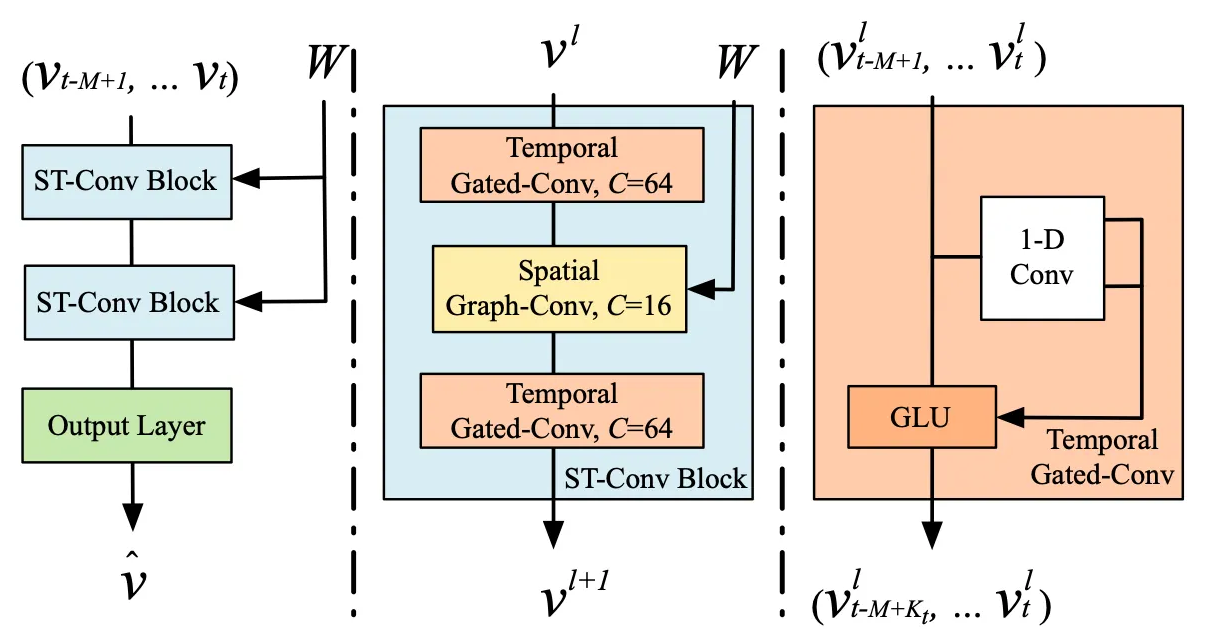
\includegraphics[width=0.8\linewidth]{../images/stgcn_model.png}
            \caption{STGCN scheme.}
        \end{figure}
    \end{frame}
    
    \begin{frame}{STGCN in action}
        \begin{figure}
            \centering
            % \includegraphics{}
            \animategraphics[width=0.85\textwidth, loop, autoplay]
            {15} % frame rate
            {../images/traffic/c389b48c98f34cce898d9c1baa2ed346LTsk9cwQTrdumRQT-} % path to figures
            {0} % start index
            {232} % end index
            \caption{Visualization of traffic}
            \vspace{-15pt}
            \caption*{\tiny From: \url{https://medium.com/stanford-cs224w/predicting-evolution-of-dynamic-graphs-7688eca1daf8}}
            %%% \label{fig:stgcn_example}
        \end{figure}
    \end{frame}

    \begin{frame}{Application in physic}
        Learning to Simulate Complex Physics with Graph Networks \cite{sanchez2020learning}.
        
        \begin{figure}[ht!]
            \centering
            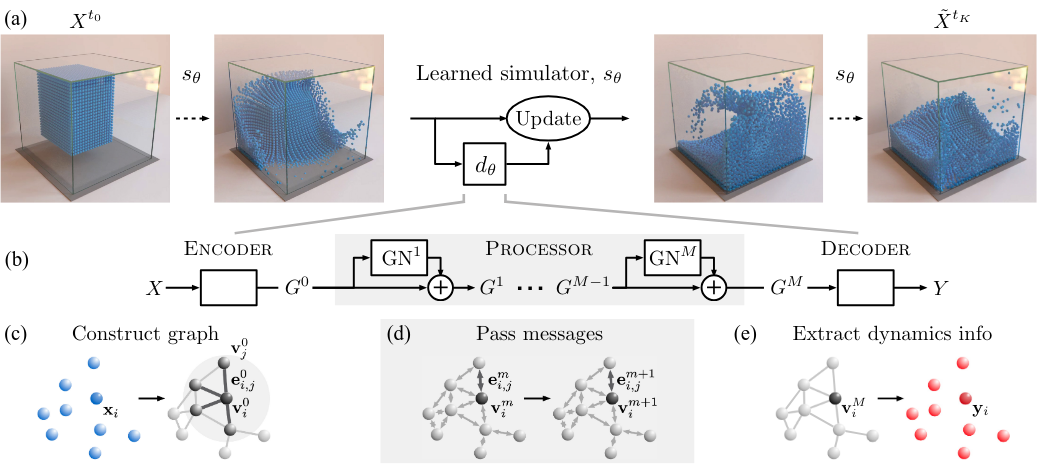
\includegraphics[width=0.9\linewidth]{../images/gns.png}
            \caption{GNS scheme.}
        \end{figure}
    \end{frame}
    
    \begin{frame}{GNS in action}
        \begin{figure}
            \centering
            % \includegraphics{}
            \animategraphics[width=0.85\textwidth, loop, autoplay]
            {10} % frame rate
            {../images/physics/96e5eb9cda094a5dacfe00a168965330KkJlbebmdYjuPPbO-} % path to figures
            {0} % start index
            {149} % end index
            \caption{Simulating complex physics.}
            \vspace{-15pt}
            \caption*{\tiny From: \url{https://medium.com/stanford-cs224w/simulating-complex-physics-with-graph-networks-step-by-step-177354cb9b05}}
            %%% \label{fig:gns_example}
        \end{figure}
    \end{frame}

    \begin{frame}{Application in recommender systems}
        Uber Eats
        \begin{figure}[ht!]
            \centering
            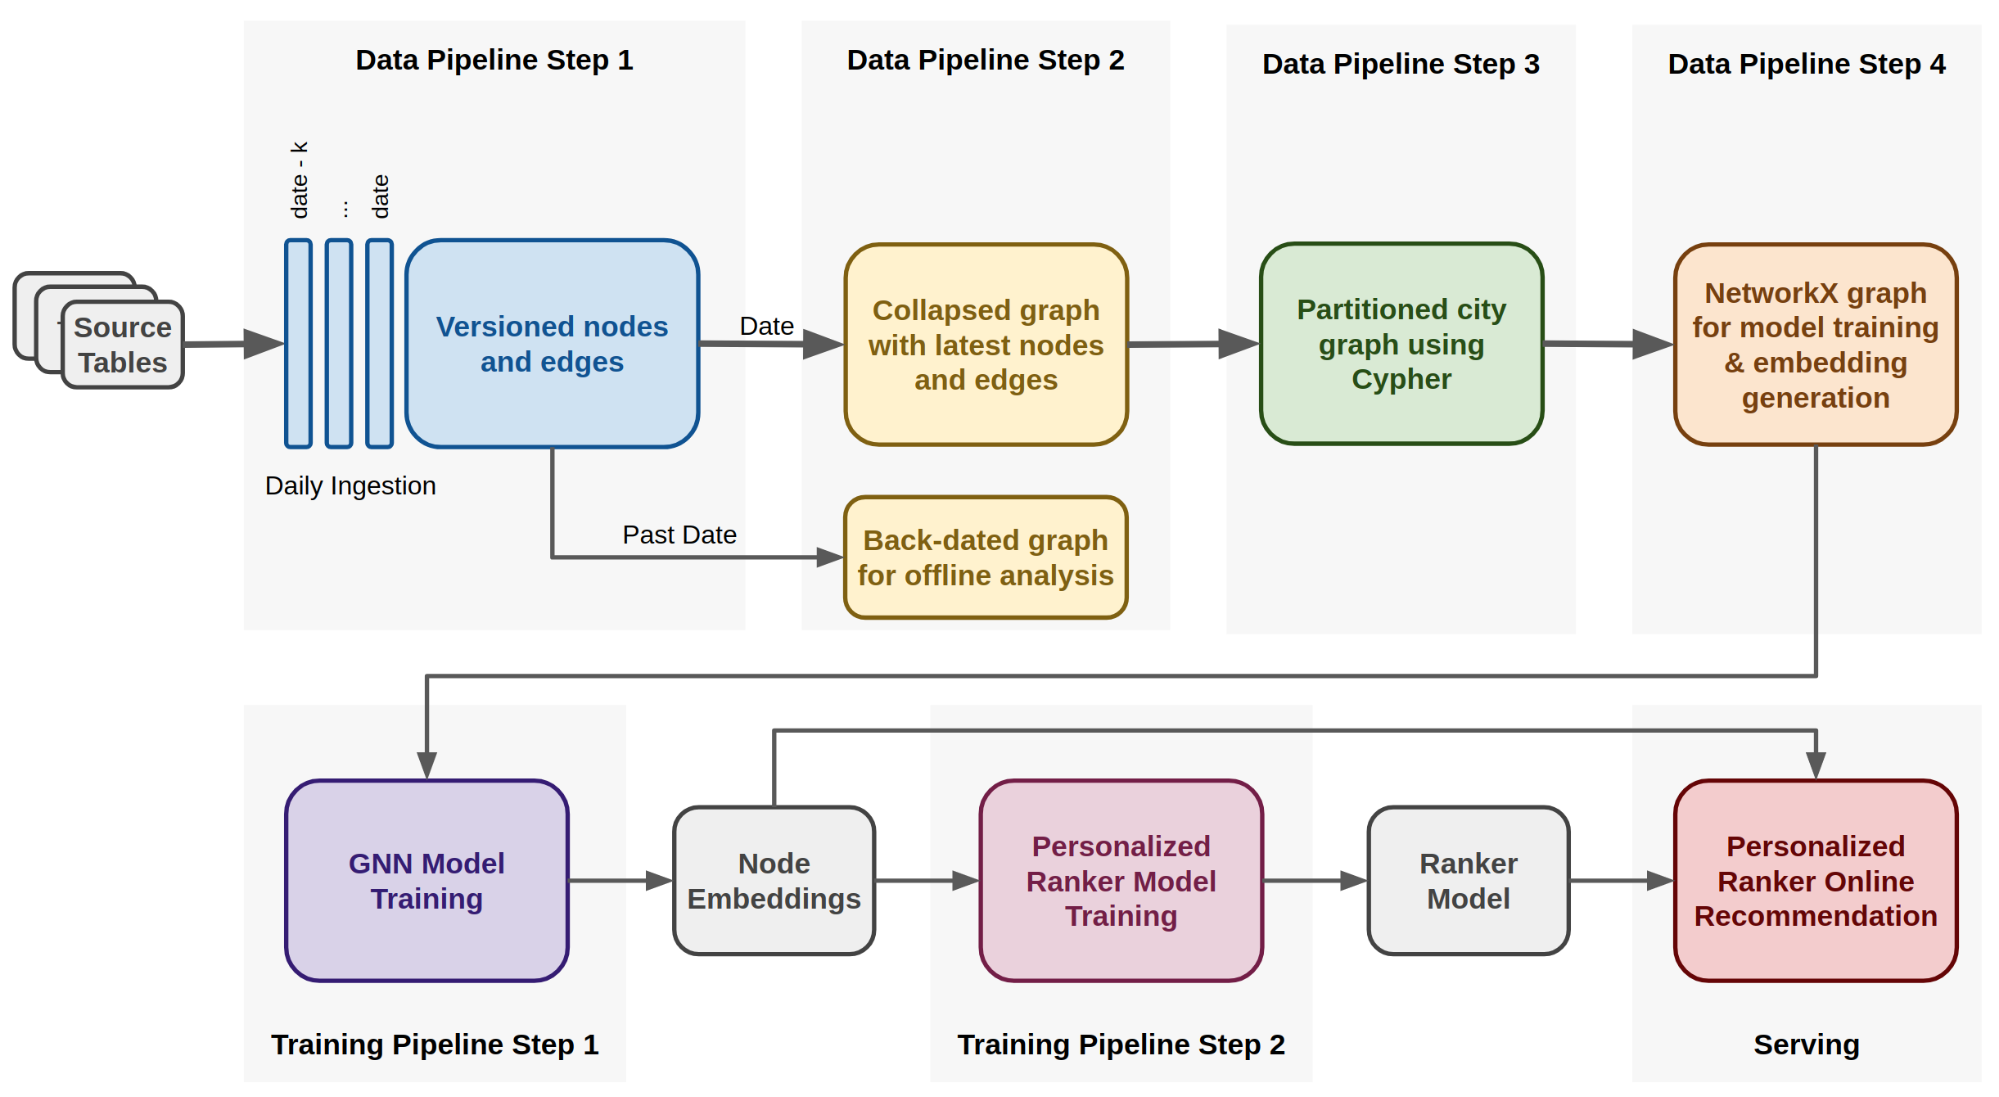
\includegraphics[width=0.9\linewidth]{../images/uber_model.png}
            \caption{Pipeline Uber eats.}
            \vspace{-15pt}
            \caption*{\tiny From: \url{https://www.uber.com/en-CO/blog/uber-eats-graph-learning/}}
        \end{figure}
    \end{frame}

    \begin{frame}{Uber Eats}
        \begin{figure}
            \centering
            % \includegraphics{}
            \animategraphics[width=0.35\textwidth, loop, autoplay]
            {5} % frame rate
            {../images/uber_eats/a733611516524151ebb9d28ad2c2ab68IaQ4dI3VB8Bs9CFt-} % path to figures
            {0} % start index
            {30} % end index
            \caption{Recommender systems app.}
            %%% \label{fig:app_ubereats}
        \end{figure}
    \end{frame}

    % \begin{frame}{Practical example: Recommending Books using LightGCN} 
    %     \begin{itemize}
    %         \item Install requirements
    %             \begin{itemize}
    %                 \item \texttt{Python}
    %                 \item \texttt{Pandas}
    %                 \item \texttt{Numpy}
    %                 \item \texttt{NetworkX}
    %                 \item \texttt{Matplotlib} / \texttt{Ploty}
    %                 \item \texttt{Scikit-learn}
    %                 \item \texttt{Torch Geometric}
    %             \end{itemize}
    %         \item Topics 
    %             \begin{itemize}
    %                 \item Recommender systems
    %             \end{itemize}
    %         \item Lab
    %             \begin{itemize}
    %                 \item              
    %                     \href{https://drive.google.com/file/d/1tY_vjLjVyBWFFzkrl7W4BFx5_y88gfdT/view?usp=sharing}{
    %                         \beamergotobutton{\faGoogle\ Open in Google Colab}
    %                     }
    %             \end{itemize}
    %     \end{itemize}
    % \end{frame}
% ---




\begin{columns}[t] % Option "c" centers vertically, while "t" aligns to the top.
    \begin{column}{0.7\textwidth}
        Given the graph $G = (V, E)$ and the node embedding matrix $Z$, compute the edge-level embeddings and graph-level embeddings: % the following node embedding matrix $Z \in \mathbb{R}^{5 \times 3}$:

        \[
            \footnotesize
            Z =
            \begin{bmatrix}
            0.5 & 0.2 & 0.8 \\
            0.1 & 0.9 & 0.4 \\
            0.6 & 0.3 & 0.7 \\
            0.2 & 0.5 & 0.1 \\
            0.8 & 0.4 & 0.6
            \end{bmatrix}
        \]

        % where each row $z_i \in \mathbb{R}^{3}$ represents the node embedding of node $i$.

        \begin{figure}[htp!]
            \centering
            
\includegraphics[
                width=0.39\linewidth,
                trim=0pt 0pt 0pt 0pt, % trim: left bottom right top
                clip
            ]{../images/union.pdf}
            \caption{Graph $G$.}
            % \source{Author, 2024.}
            % \label{fig:my_image}
        \end{figure}
    \end{column}
    \begin{column}{0.3\textwidth}

    \end{column}
\end{columns}